\chapter{Search for H(Inv) decays in the VBF channel with CMS parked data}
\label{CHAPTER:ParkedDataAnalysis}

\glsresetall % Resetting all acronyms

This chapter describes the analysis performed over the \gls{CMS} Run I parked data collected over 2012 and 2013. This data was collected and stored without reconstruction and only became fully available a few months after data taking was finished. The advantage of this dataset is the possibility to use lower threshold triggers which can collect more signal but also more backgrounds. To take full advantage of this data the analysis had to be redesigned and extended with new control regions.

% The search for an invisible decay of a vector boson produced Higgs boson was first made public with CMS Physics Analysis Summary (PAS) HIG-13-013 which was further improved and combined with other Higgs boson production channel in the CMS paper HIG-13-30. Additional support material can be found at the CMS Analysis Notes (AN) AN-2012/403 \cite{CMS_AN_2013-403} and AN-2013/205.
% 
% During the 2012 data taking run two main streams of data were recorded. The main stream with an event rate of the order of 300 Hz to be promptly reconstructed and made available for analysis in a few days after being recorded, this dataset is referred to as the prompt data. The secondary stream with lower trigger thresholds with an event rate of the order of 1kHz which would only be reconstructed when the computing resources would be available outside of the data taking period, dataset is referred to as parked data. Our previous results
% were produced using the prompt data only and this work now extends on previous work by using the now available parked data. Since this dataset has been recorded with lower trigger thresholds the analysis was re-optimised to take advantage of this new available phase space. The details of the newly developed analysis can be found in CMS AN-14-243\cite{CMS_AN_2014-243}.
% 
%TODO: references? previous chapter?

%%%%%%%%%%%%%%%%%%%%%%%%%%%%%%%%%%%%%%%%%%%%%%%%%%%%%%%%%%%%%%%%%%%%%%%%%%%%%%%%%%%%
%%% SECTION
%%%%%%%%%%%%%%%%%%%%%%%%%%%%%%%%%%%%%%%%%%%%%%%%%%%%%%%%%%%%%%%%%%%%%%%%%%%%%%%%%%%%
\section{The Cross Check Analysis}
\label{CHAPTER:ParkedDataAnalysis_CrossCheckAnalysis}

%Status: DONE

It is normally a requirement for many CMS publications to have a cross check analysis implemented independently from the main result in order to be able to ensure accuracy of the final results due to possible errors with the software implementation. For this purpose the previous prompt data \gls{VBF} Higgs to Invisible results and publication were produced by two different and independent code frameworks and before publication a good level of synchronization was obtained. Due to lack of man power and time it was decide for the 2012-13 parked data analysis to only proceed with a single framework. At a later stage of the analysis it was thought that at least some level of cross check would be a good measure to limit the possibility of implementation errors and to allow extra confidence on the final results.
 
This cross check analysis starts from the same ntuples produced by the main analysis which were produced over all the relevant datasets. This ntuples are recorded with data formats also used by other analysis at Imperial College London, e.g. both the \gls{SM} and \gls{MSSM} Higgs to $\tau\bar{\tau}$, the Higgs to $\tau\bar{\tau}b\bar{b}$ and prompt Higgs to invisible analyses. No cuts are applied at ntuple production except the official \gls{CMS} selection for good usable data using the appropriate golden \gls{JSON} file.
 
To analyse those initial ntuple an independent code framework was developed in order to replicate all relevant numbers and plots produced by the main analysis.


%%%%%%%%%%%%%%%%%%%%%%%%%%%%%%%%%%%%%%%%%%%%%%%%%%%%%%%%%%%%%%%%%%%%%%%%%%%%%%%%%%%%
%%% SECTION
%%%%%%%%%%%%%%%%%%%%%%%%%%%%%%%%%%%%%%%%%%%%%%%%%%%%%%%%%%%%%%%%%%%%%%%%%%%%%%%%%%%%
\section{Data and MC samples}

%%%%%%%%%%%%%%%%%%%%%%%%%%%%%%%%%%%%%%%%%%%%%%%%%%%%%%%%%%%%%%%%%%%%%%%%%%%%%%%%%%%%
%%% SUBSECTION
%%%%%%%%%%%%%%%%%%%%%%%%%%%%%%%%%%%%%%%%%%%%%%%%%%%%%%%%%%%%%%%%%%%%%%%%%%%%%%%%%%%%
\subsection{Data}

%Status: DONE

In this analysis we used the full certified data with collisions at $\sqrt{s}=8\,\TeV$ from 2012-13 data acquisition (Run I), using golden \gls{JSON} file:

\begin{verbatim}
Cert_190456-208686_8TeV_22Jan2013ReReco_Collisions12_JSON.txt
\end{verbatim}

It amounts to an integrated luminosity of $19.2 \pm 0.5 \,\femto\barn^{-1}$. A summary of the dataset names and their integrated luminosity can be found in table \ref{TABLE:ParkedData_Data_RunI_IntegratedLuminosity}.

\begin{table}[!htb]
\centering
\begin{tabular}{|c|c|c|}
\hline
Era & Type & $\int{Luminosity}$ $[pb^{-1}]$ \\
\hline \hline
Run A & Prompt Data &  889 \\
Run B & Parked Data & 3871 \\
Run C & Parked Data & 7152 \\
Run D & Parked Data & 7317 \\
\hline\hline
\multicolumn{2}{|c|}{Total analysed} & 19229 \\
\hline\hline
\multicolumn{2}{|c|}{Total certified luminosity} & 19789 \\
\hline
\end{tabular}
\caption{Relevant parked datasets from Run I and their total analysed integrated luminosity. Total analysed and certified also showed.}
\label{TABLE:ParkedData_Data_RunI_IntegratedLuminosity}
\end{table}


The difference between certified and analysed numbers is due to our analysis trigger not being active for the first few runs of of Run 2012B.

%%%%%%%%%%%%%%%%%%%%%%%%%%%%%%%%%%%%%%%%%%%%%%%%%%%%%%%%%%%%%%%%%%%%%%%%%%%%%%%%%%%%
%%% SUBSECTION
%%%%%%%%%%%%%%%%%%%%%%%%%%%%%%%%%%%%%%%%%%%%%%%%%%%%%%%%%%%%%%%%%%%%%%%%%%%%%%%%%%%%
\subsection{Monte Carlo Samples}

% \resizebox{1.00\linewidth}{!}{
\begin{longtable}{| l | c | c | c |}
  \caption{\label{tab:MCSamples} MC processes, corresponding cross sections (at NLO or NNLO when available) and equivalent integrated
    luminosity analysed.} \\
  \hline 
  Dataset & $\sigma$ [pb] & No. of Events & Equivalent $\int L$ [fb$^{-1}$] \\
  \hline 
  ($Z \rightarrow \nu\nu$) + jets (50 $<$ HT $<$ 100 GeV)       & 381.2         &  4040980 &    10.6 \\
  ($Z \rightarrow \nu\nu$) + jets (100 $<$ HT $<$ 200 GeV)      & 160.3         &  4416646 &    27.6 \\
  ($Z \rightarrow \nu\nu$) + jets (200 $<$ HT $<$ 400 GeV)      & 41.49         &  5055885 &     122 \\
  ($Z \rightarrow \nu\nu$) + jets (400 $<$ HT $<$ $\infty$ GeV) & 5.274         &  1006928 &     191 \\
  ($W \rightarrow l\nu$) + jets (inclusive)                     & 37509(NNLO)   & 76102995 &    2.03 \\
  ($W \rightarrow l\nu$) + 1 jet                                & 5400          & 23141598 &    42.9 \\
  ($W \rightarrow l\nu$) + 2 jet                                & 1750          & 34044921 &    19.5 \\
  ($W \rightarrow l\nu$) + 3 jet                                & 519           & 15539503 &    29.9 \\
  ($W \rightarrow l\nu$) + 4 jet                                & 214           & 13382803 &    62.5 \\
  ($Z/\gamma \rightarrow ll$) + jets (Mll $>$ 50)               & 3503.71(NNLO) & 30459503 &     8.7 \\
  ($Z/\gamma \rightarrow ll$) + 1 jets (Mll $>$ 50)             & 561           & 24045248 &    42.9 \\
  ($Z/\gamma \rightarrow ll$) + 2 jets (Mll $>$ 50)             & 181           & 21852156 &     121 \\
  ($Z/\gamma \rightarrow ll$) + 3 jets (Mll $>$ 50)             & 51.1          & 11015445 &     216 \\
  ($Z/\gamma \rightarrow ll$) + 4 jets (Mll $>$ 50)             & 23.04         &  6402827 &     278 \\
  EWK ($Z/\gamma \rightarrow ll$) + 2 jets                      & 0.888         &  2978717 &    3354 \\
  EWK ($W^{+} \rightarrow l\nu$) + 2 jets                       & 6.48          &  8996164 &    1388 \\
  EWK ($W^{-} \rightarrow l\nu$) + 2 jets                       & 4.09          &  5994018 &    1466 \\ 
  WW                                                            & 54.838(NLO)   & 10000431 &     182 \\
  WZ                                                            & 33.21(NLO)    & 10000283 &     301 \\
  ZZ                                                            & 17.654(NLO)   &  9799908 &     555 \\
  $W \gamma$                                                    & 461.6         &  4802358 &    10.4 \\
  tt + jets                                                     & 245.8(NNLO)   &  6923750 &    28.2 \\
  t (t-channel)                                                 & 56.4(NLO)     &  3758227 &    66.6 \\
  t (tW-channel)                                                & 11.1(NLO)     &   497658 &    44.8 \\
  t (s-channel)                                                 & 3.79(NLO)     &   259961 &    68.6 \\
  $\bar{t}$ (t-channel)                                         & 30.7(NLO      &  1935072 &    63.0 \\
  $\bar{t}$ (tW-channel)                                        & 11.1(NLO)     &   493460 &    44.5 \\
  $\bar{t}$ (s-channel)                                         & 1.76(NLO)     &   139974 &    79.5 \\
  QCD (30 $<$ p T $<$ 50 GeV)                                   & 66285328.0    &  6000000 & 0.00009 \\
  QCD (50 $<$ p T $<$ 80 GeV)                                   & 8148778.0     &  5998860 & 0.00074 \\
  QCD (80 $<$ p T $<$ 120 GeV)                                  & 1033680.0     &  5994864 &  0.0058 \\
  QCD (120 $<$ p T $<$ 170 GeV)                                 & 156293.3      &  5985732 &   0.038 \\
  QCD (170 $<$ p T $<$ 300 GeV)                                 & 34138.15      &  5814398 &   0.170 \\
  QCD (300 $<$ p T $<$ 470 GeV)                                 & 1759.549      &  5978500 &    3.40 \\
  QCD (470 $<$ p T $<$ 600 GeV)                                 & 113.8791      &  3964848 &    34.8 \\
  QCD (600 $<$ p T $<$ 800 GeV)                                 & 26.9921       &  3996864 &     148 \\
  QCD (800 $<$ p T $<$ 1000 GeV)                                & 3.550036      &  3998563 &    1130 \\
  QCD (1000 $<$ p T $<$ 1400 GeV)                               & 0.737844      &   964088 &    1310 \\
  QCD (1400 $<$ p T $<$ 1800 GeV)                               & 0.03352235    &  2000062 &   60000 \\
  QCD (1800 $<$ p T $<$ $\infty$ GeV)                           & 0.001829005   &   977586 &  534000 \\
  \hline
\end{longtable}
% }

%%%%%%%%%%%%%%%%%%%%%%%%%%%%%%%%%%%%%%%%%%%%%%%%%%%%%%%%%%%%%%%%%%%%%%%%%%%%%%%%%%%%
%%% SECTION
%%%%%%%%%%%%%%%%%%%%%%%%%%%%%%%%%%%%%%%%%%%%%%%%%%%%%%%%%%%%%%%%%%%%%%%%%%%%%%%%%%%%
\section{Monte Carlo to Data correction factors}

%Status: DONE

To correctly compare \gls{MC} with data all relevant aspects must be correctly taken into account. In the event that a variable distribution does not match between both we can determine weights to apply to each event so the distributions match again. In these analysis we apply four weights to \gls{MC}, to obtain the correct \gls{PU} distribution, weight events according to the probability of passing the trigger, account for lepton identification probability and top sample re-weghting.

%%%%%%%%%%%%%%%%%%%%%%%%%%%%%%%%%%%%%%%%%%%%%%%%%%%%%%%%%%%%%%%%%%%%%%%%%%%%%%%%%%%%
%%% SUBSECTION
%%%%%%%%%%%%%%%%%%%%%%%%%%%%%%%%%%%%%%%%%%%%%%%%%%%%%%%%%%%%%%%%%%%%%%%%%%%%%%%%%%%%
\subsection{Pile-up}

%%%%%%%%%%%%%%%%%%%%%%%%%%%%%%%%%%%%%%%%%%%%%%%%%%%%%%%%%%%%%%%%%%%%%%%%%%%%%%%%%%%%
%%% SUBSECTION
%%%%%%%%%%%%%%%%%%%%%%%%%%%%%%%%%%%%%%%%%%%%%%%%%%%%%%%%%%%%%%%%%%%%%%%%%%%%%%%%%%%%
\subsection{Trigger efficiency}
\label{SUBSECTION:ParkedDataAnalysis_CorrectionFactors_TriggerEfficiency}

%Status: DONE

The initial event selection for this analysis starts with a dedicated set of triggers which were recorded to the \gls{VBF} parked dataset. We used the following \gls{HLT} trigger paths for each Run I era:

\begin{itemize}
  \item Run A:       \verb!HLT_DiPFJet40_PFMETnoMu65_MJJ800VBF_AllJets!
  \item Run B and C: \verb!HLT_DiJet35_MJJ700_AllJets_DEta3p5_VBF!
  \item Run D:       \verb!HLT_DiJet30_MJJ700_AllJets_DEta3p5!
\end{itemize}

All the used paths are seeded by \gls{L1T} trigger condition \verb!L1_ETM40!. 

To maximize the usage of the event statistics of the selected \gls{MC} samples, we do not veto events that fail the trigger conditions. Instead an event by event weight is calculated which which taking into account how much luminosity was recorded by each of the three trigger and depending on the offline quantities which correspond to the ones used in the trigger conditions: PFMETnoMu, leading dijet $m_{jj}$ and sub-leading jet \pt. 

To define the weights, turn on curves were determined according to these offline variables as a function of PFMETnoMu in bins of dijet $m_{jj}$ and sub-leading jet \pt. This approach allows the determination of the weights which include the correlations between these variables. The turn on curves are obtained by fitting equation \ref{EQUATION:ParkedDataAnalysis_TriggerEfficiency_Efficiency} to each bin.

\begin{equation}
\frac{\varepsilon_{max}}{2}\text{Erf}\left(\frac{x-x_{0}}{\sqrt{\Gamma}}\right)+1,
\label{EQUATION:ParkedDataAnalysis_TriggerEfficiency_Efficiency} 
\end{equation}

Where $\varepsilon_{max}$ os the maximum efficiency of the trigger in the bin, $x_{0}$ is the mid-value of the turn on and $\Gamma$ is the width of the turn on.

%%%%%%%%%%%%%%%%%%%%%%%%%%%%%%%%%%%%%%%%%%%%%%%%%%%%%%%%%%%%%%%%%%%%%%%%%%%%%%%%%%%%
%%% SUBSECTION
%%%%%%%%%%%%%%%%%%%%%%%%%%%%%%%%%%%%%%%%%%%%%%%%%%%%%%%%%%%%%%%%%%%%%%%%%%%%%%%%%%%%
\subsection{Lepton Identification}

%%%%%%%%%%%%%%%%%%%%%%%%%%%%%%%%%%%%%%%%%%%%%%%%%%%%%%%%%%%%%%%%%%%%%%%%%%%%%%%%%%%%
%%% SUBSECTION
%%%%%%%%%%%%%%%%%%%%%%%%%%%%%%%%%%%%%%%%%%%%%%%%%%%%%%%%%%%%%%%%%%%%%%%%%%%%%%%%%%%%
\subsection{Top reweighting}

%%%%%%%%%%%%%%%%%%%%%%%%%%%%%%%%%%%%%%%%%%%%%%%%%%%%%%%%%%%%%%%%%%%%%%%%%%%%%%%%%%%%
%%% SECTION
%%%%%%%%%%%%%%%%%%%%%%%%%%%%%%%%%%%%%%%%%%%%%%%%%%%%%%%%%%%%%%%%%%%%%%%%%%%%%%%%%%%%
\section{Signal event selection}


\begin{table}[htp]
\centering
\begin{tabular}{|l|c|c|c|c||c|}
\hline
 & \rotatebox{90}{Prompt Run A} & \rotatebox{90}{Parked Run B} & \rotatebox{90}{Parked Run C} & \rotatebox{90}{Parked Run D} & \rotatebox{90}{Total Data} \\
\hline \hline
Vertex Filter                   & 3606391 & 132346320 & 228049748 & 308041846 & 672044305 \\
Event Quality Filters           & 2658960 & 131554431 & 226680352 & 305918529 & 666812272 \\
ECAL Laser Filter               & 2634271 & 131543040 & 226680352 & 305918529 & 666776192 \\
HCAL Laser Filter               & 2634080 & 131543040 & 226679741 & 305918529 & 666775390 \\
L1T ETM Filter                  & 2461217 &  88174347 & 160560859 & 227801622 & 478998045 \\
HLT Filter                      &   97522 &  75100422 & 137527238 & 152041761 & 364766943 \\
$N(Electrons_{veto})=0$         &   96600 &  74947192 & 137241812 & 151725585 & 364011189 \\
$N(Muon_{loose})=0$             &   94864 &  74913002 & 137179173 & 151652654 & 363839693 \\
Dijet cut                       &   18338 &  13678405 &  25090291 &  24082304 &  62869338 \\
MET cut                         &    4167 &     38178 &     68047 &     79723 &    190115 \\
$MET_{Significance}$ cut        &     786 &      3396 &      5988 &      5567 &     15737 \\
$Min(\Delta\phi(MET,jets))$ cut &      34 &        91 &       205 &       178 &       508 \\
\hline
\end{tabular}
\caption{Event Yield for the Signal Region.}
\end{table}



%%%%%%%%%%%%%%%%%%%%%%%%%%%%%%%%%%%%%%%%%%%%%%%%%%%%%%%%%%%%%%%%%%%%%%%%%%%%%%%%%%%%
%%% SECTION
%%%%%%%%%%%%%%%%%%%%%%%%%%%%%%%%%%%%%%%%%%%%%%%%%%%%%%%%%%%%%%%%%%%%%%%%%%%%%%%%%%%%
\section{Control Regions}

%%%%%%%%%%%%%%%%%%%%%%%%%%%%%%%%%%%%%%%%%%%%%%%%%%%%%%%%%%%%%%%%%%%%%%%%%%%%%%%%%%%%
%%% SUBSECTION
%%%%%%%%%%%%%%%%%%%%%%%%%%%%%%%%%%%%%%%%%%%%%%%%%%%%%%%%%%%%%%%%%%%%%%%%%%%%%%%%%%%%
\subsection{Top background estimation}

%%%%%%%%%%%%%%%%%%%%%%%%%%%%%%%%%%%%%%%%%%%%%%%%%%%%%%%%%%%%%%%%%%%%%%%%%%%%%%%%%%%%
%%% SUBSECTION
%%%%%%%%%%%%%%%%%%%%%%%%%%%%%%%%%%%%%%%%%%%%%%%%%%%%%%%%%%%%%%%%%%%%%%%%%%%%%%%%%%%%
\subsection{W background estimation}

%%%%%%%%%%%%%%%%%%%%%%%%%%%%%%%%%%%%%%%%%%%%%%%%%%%%%%%%%%%%%%%%%%%%%%%%%%%%%%%%%%%%
%%% SUBSECTION
%%%%%%%%%%%%%%%%%%%%%%%%%%%%%%%%%%%%%%%%%%%%%%%%%%%%%%%%%%%%%%%%%%%%%%%%%%%%%%%%%%%%
\subsection{W background estimation}

%%%%%%%%%%%%%%%%%%%%%%%%%%%%%%%%%%%%%%%%%%%%%%%%%%%%%%%%%%%%%%%%%%%%%%%%%%%%%%%%%%%%
%%% SUBSUBSECTION
%%%%%%%%%%%%%%%%%%%%%%%%%%%%%%%%%%%%%%%%%%%%%%%%%%%%%%%%%%%%%%%%%%%%%%%%%%%%%%%%%%%%
\subsubsection{W to electron+neutrino}

%%%%%%%%%%%%%%%%%%%%%%%%%%%%%%%%%%%%%%%%%%%%%%%%%%%%%%%%%%%%%%%%%%%%%%%%%%%%%%%%%%%%
%%% SUBSUBSECTION
%%%%%%%%%%%%%%%%%%%%%%%%%%%%%%%%%%%%%%%%%%%%%%%%%%%%%%%%%%%%%%%%%%%%%%%%%%%%%%%%%%%%
\subsubsection{W to muon+neutrino}

%%%%%%%%%%%%%%%%%%%%%%%%%%%%%%%%%%%%%%%%%%%%%%%%%%%%%%%%%%%%%%%%%%%%%%%%%%%%%%%%%%%%
%%% SUBSUBSECTION
%%%%%%%%%%%%%%%%%%%%%%%%%%%%%%%%%%%%%%%%%%%%%%%%%%%%%%%%%%%%%%%%%%%%%%%%%%%%%%%%%%%%
\subsubsection{W to tau+neutrino}

%%%%%%%%%%%%%%%%%%%%%%%%%%%%%%%%%%%%%%%%%%%%%%%%%%%%%%%%%%%%%%%%%%%%%%%%%%%%%%%%%%%%
%%% SUBSECTION
%%%%%%%%%%%%%%%%%%%%%%%%%%%%%%%%%%%%%%%%%%%%%%%%%%%%%%%%%%%%%%%%%%%%%%%%%%%%%%%%%%%%
\subsection{Z background estimation}

%%%%%%%%%%%%%%%%%%%%%%%%%%%%%%%%%%%%%%%%%%%%%%%%%%%%%%%%%%%%%%%%%%%%%%%%%%%%%%%%%%%%
%%% SUBSECTION
%%%%%%%%%%%%%%%%%%%%%%%%%%%%%%%%%%%%%%%%%%%%%%%%%%%%%%%%%%%%%%%%%%%%%%%%%%%%%%%%%%%%
\subsection{QCD background estimation}

%%%%%%%%%%%%%%%%%%%%%%%%%%%%%%%%%%%%%%%%%%%%%%%%%%%%%%%%%%%%%%%%%%%%%%%%%%%%%%%%%%%%
%%% SUBSUBSECTION
%%%%%%%%%%%%%%%%%%%%%%%%%%%%%%%%%%%%%%%%%%%%%%%%%%%%%%%%%%%%%%%%%%%%%%%%%%%%%%%%%%%%
\subsubsection{QDC VBF-like + MET Monte Carlo Sample}

%%%%%%%%%%%%%%%%%%%%%%%%%%%%%%%%%%%%%%%%%%%%%%%%%%%%%%%%%%%%%%%%%%%%%%%%%%%%%%%%%%%%
%%% SUBSUBSECTION
%%%%%%%%%%%%%%%%%%%%%%%%%%%%%%%%%%%%%%%%%%%%%%%%%%%%%%%%%%%%%%%%%%%%%%%%%%%%%%%%%%%%
\subsubsection{Data driven QCD estimation}

%%%%%%%%%%%%%%%%%%%%%%%%%%%%%%%%%%%%%%%%%%%%%%%%%%%%%%%%%%%%%%%%%%%%%%%%%%%%%%%%%%%%
%%% SECTION
%%%%%%%%%%%%%%%%%%%%%%%%%%%%%%%%%%%%%%%%%%%%%%%%%%%%%%%%%%%%%%%%%%%%%%%%%%%%%%%%%%%%
\section{Systematics}

\begin{table}[!htb]
\centering
\label{tab:syst-qqH}
\begin{tabular}{lcc}
\hline \hline
Source  & Total background & Signal     \\
\hline
Control region data stat. & 9.3 & - \\
MC stat. & 5.4 & 3.8 \\
Jet energy scale & 4.6 & 11 \\ 
$W\rightarrow\tau\nu$ control region extrapolation & 4.3 & - \\ 
QCD normalisation & 3.2 & - \\ 
Jet energy resolution & 3.0 & 1.8 \\ 
Lepton ID efficiency & 2.4 & - \\ 
Unclustered energy scale & 1.9 & 1.6 \\ 
Pileup weight & 1.1 & 1.5 \\ 
Top MC scale factor unc. & 0.25 & - \\ 
Luminosity & 0.02 & 2.6 \\ 
QCD scale, PDF and cross section uncertainties & 0.01 & 5.2 \\
\hline \hline
\end{tabular}
\caption{Summary of the uncertainties on the total background and signal yields. All uncertainties affect the normalization of the yield, and are quoted as the change in \% in the total background or signal estimate, when each systematic effect is varied according to its uncertainties. The signal uncertainties are given for $m_H=125$\GeV and $\BRinv=100$\%.}
\end{table}

%%%%%%%%%%%%%%%%%%%%%%%%%%%%%%%%%%%%%%%%%%%%%%%%%%%%%%%%%%%%%%%%%%%%%%%%%%%%%%%%%%%%
%%% SECTION
%%%%%%%%%%%%%%%%%%%%%%%%%%%%%%%%%%%%%%%%%%%%%%%%%%%%%%%%%%%%%%%%%%%%%%%%%%%%%%%%%%%%
\section{Results}

\begin{tabular}{lc}
\hline \hline
Process & Event yields \\
\hline
$Z\rightarrow\nu\nu$&$158.1 \pm 37.3 \pm 21.2$\\
$W\rightarrow\mu\nu$&$102.5 \pm 6.2 \pm 11.7$\\
$W\rightarrow e\nu$&$57.9 \pm 7.4 \pm 7.7$\\
$W\rightarrow\tau\nu$&$94.6 \pm 13.1 \pm 23.8$\\
top&$5.5 \pm  1.8$\\
VV&$3.9 \pm 0.7$\\
QCD multijet &$17\pm 14$\\
\hline
Total Background &$439.4 \pm 40.7 \pm 43.5 $\\
\hline
Signal(VBF) &$273.1 \pm 31.2 $\\
Signal(ggH) &$23.1 \pm 15.9 $\\
\hline
Observed data & 508 \\
\hline \hline
\end{tabular}

\subsection{Comparison with the cross-check analysis}

%%%%%%%%%%%%%%%%%%%%%%%%%%%%%%%%%%%%%%%%%%%%%%%%%%%%%%%%%%%%%%%%%%%%%%%%%%%%%%%%%%%%
%%% SECTION
%%%%%%%%%%%%%%%%%%%%%%%%%%%%%%%%%%%%%%%%%%%%%%%%%%%%%%%%%%%%%%%%%%%%%%%%%%%%%%%%%%%%
\section{Extraction of limits}

\begin{figure}[h!]
  \begin{center}
    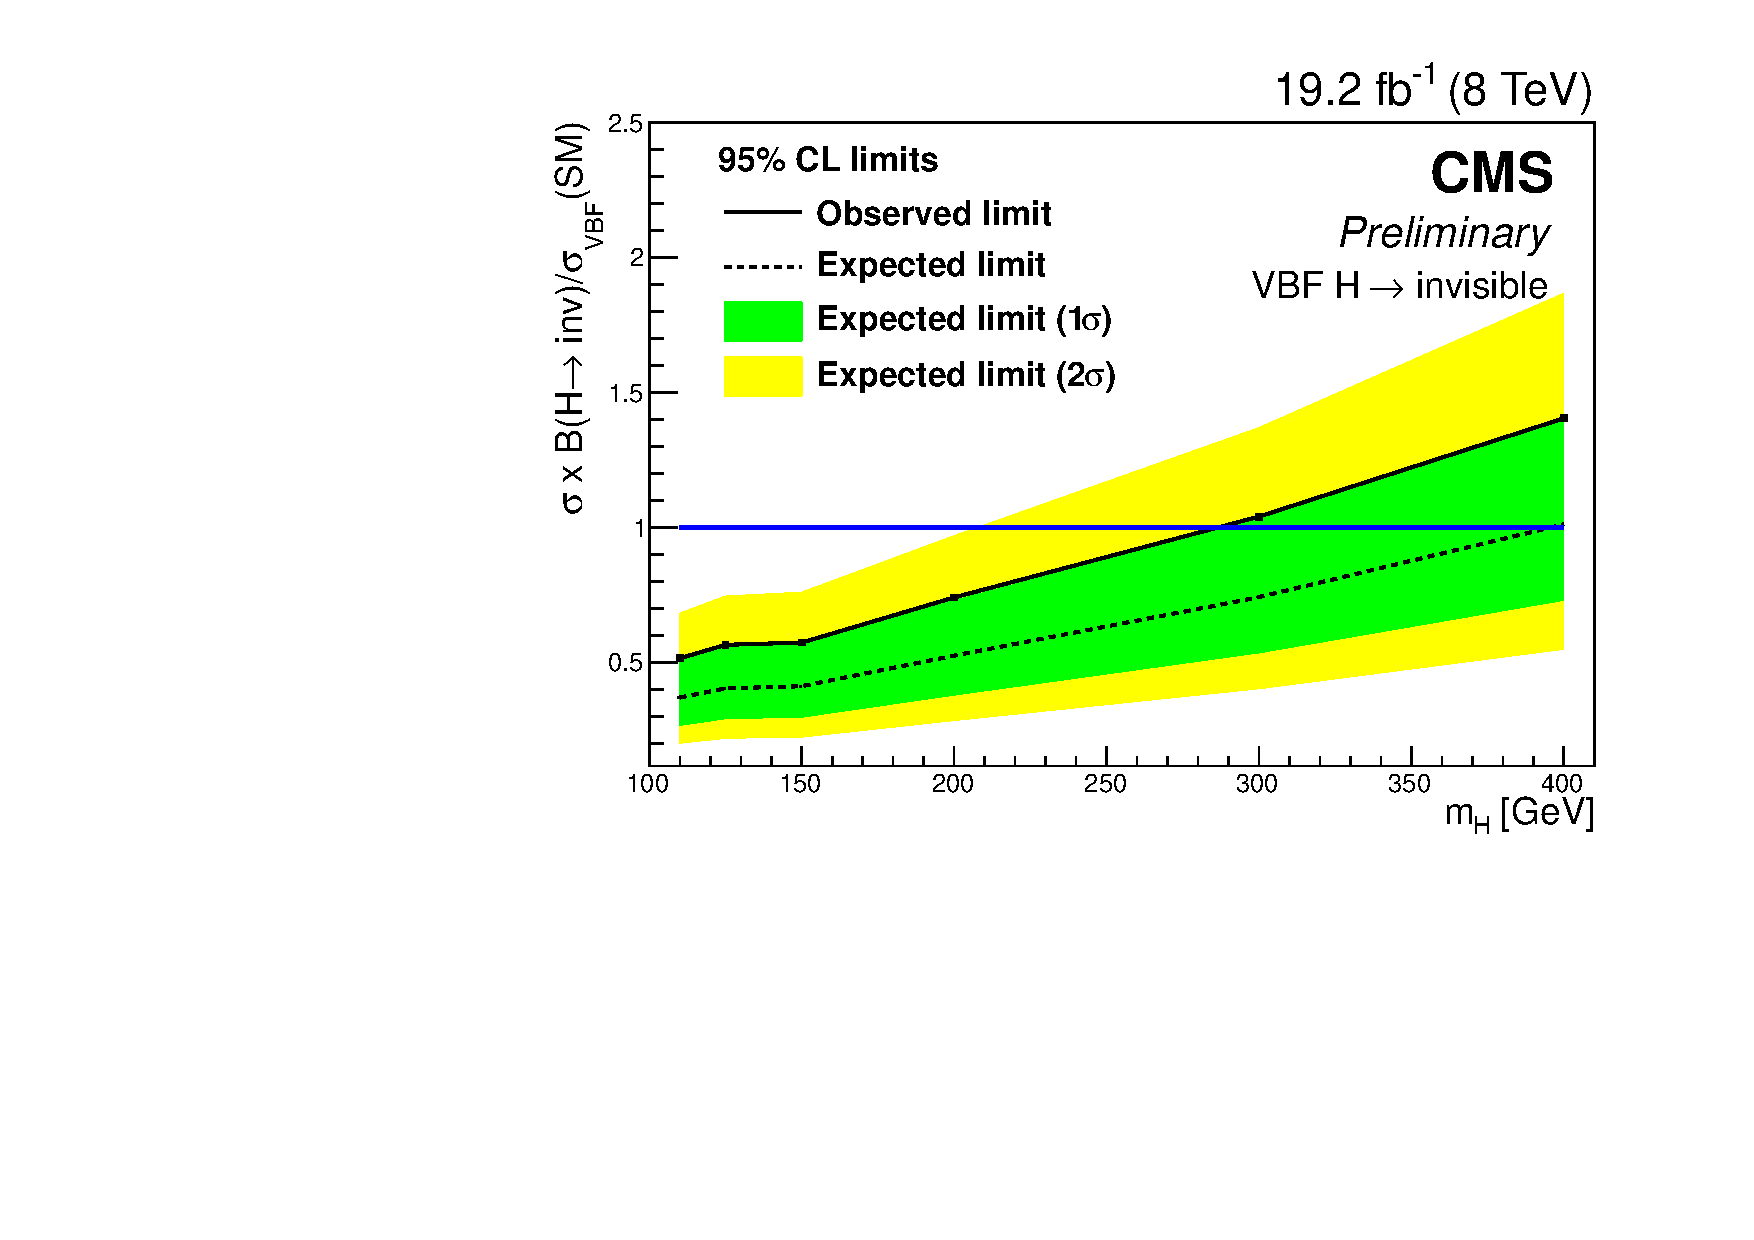
\includegraphics[width=0.49\textwidth]{Chapter07/Images/vbflimit.pdf} %!!UNBLIND ALREADY IN                                                                       
    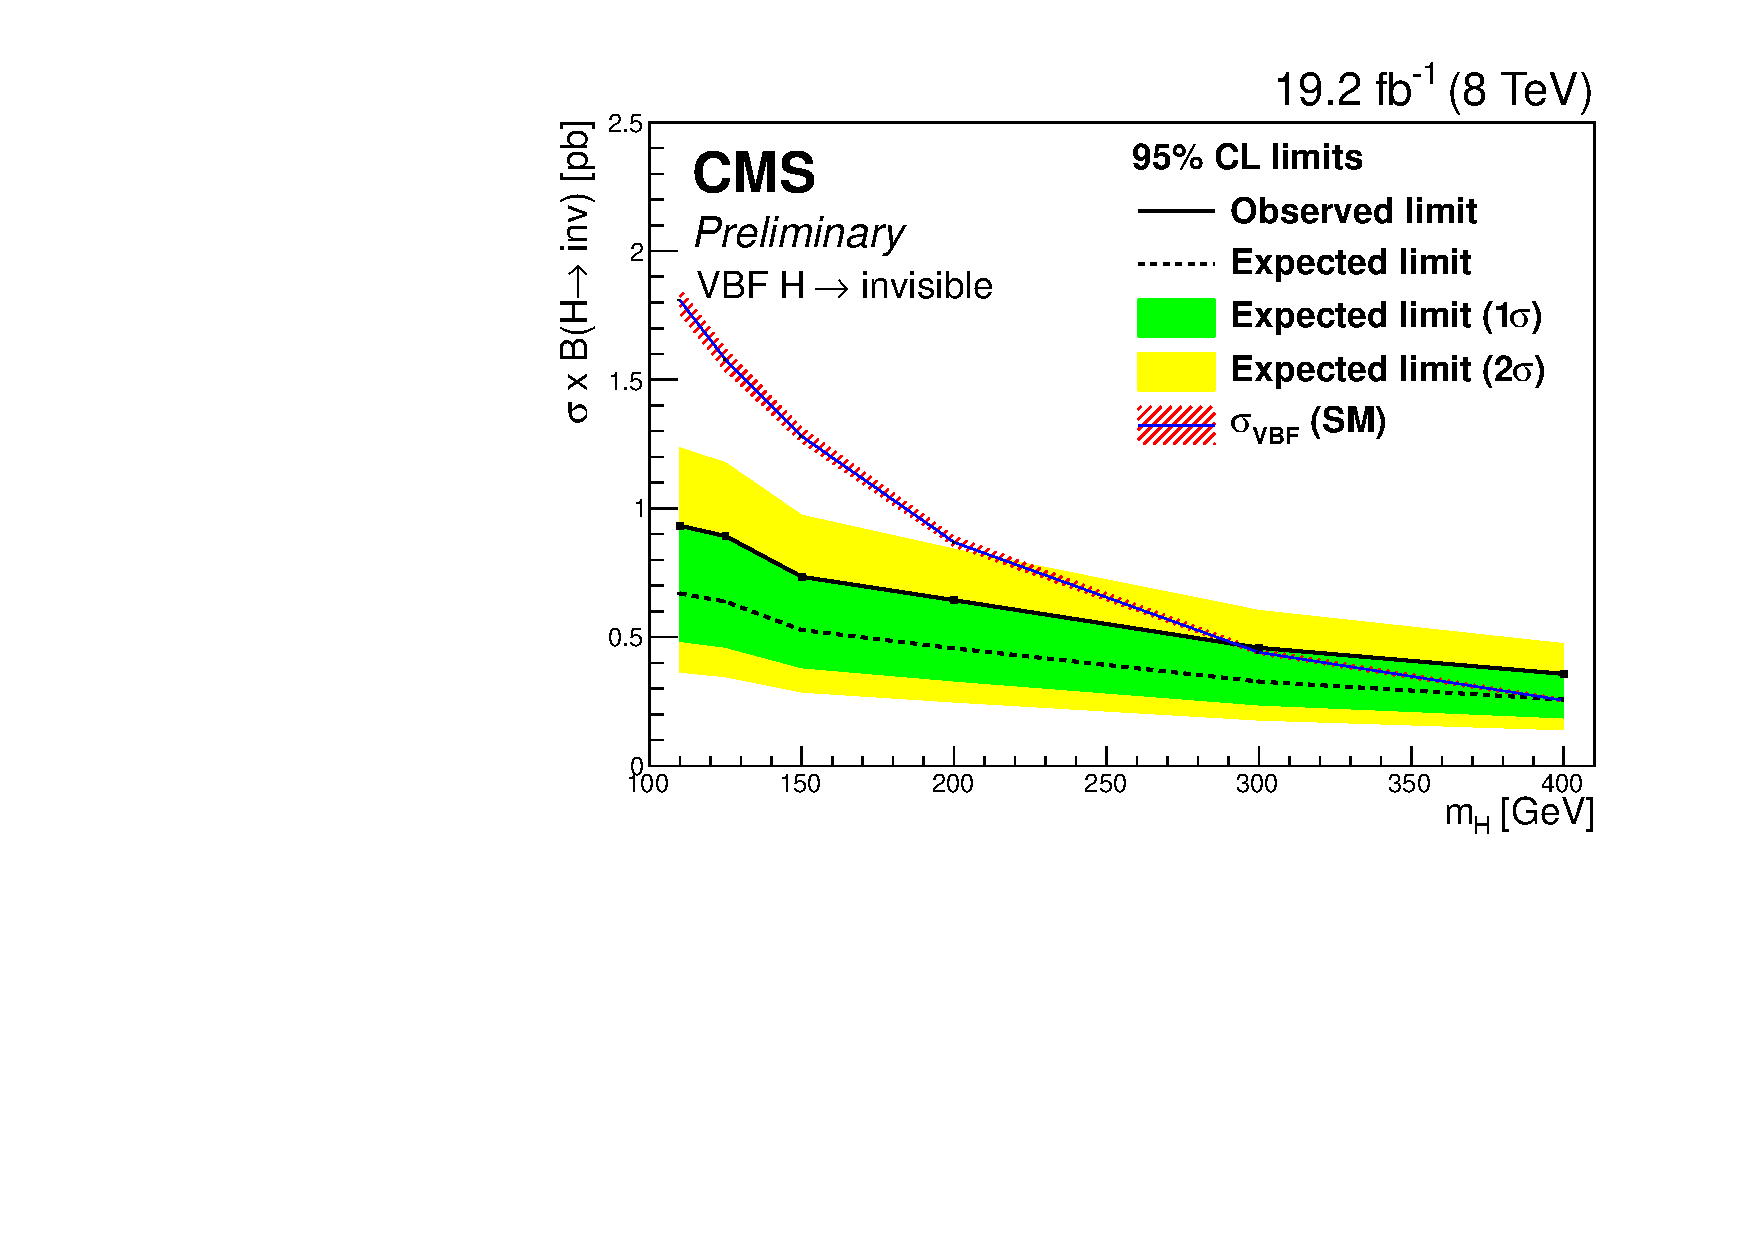
\includegraphics[width=0.49\textwidth]{Chapter07/Images/vbfxslimit.pdf}
 \caption{The 95\% C.L. limit on \BRinv\, of a SM Higgs
boson (left) and the 95\% C.L. limit on the cross section times
\BRinv\, (right)as a function of the Higgs
boson mass, assuming SM Higgs boson acceptances.}
    \label{fig:limits}
  \end{center}
\end{figure}

% %%%%%%%%%%%%%%%%%%%%%%%%%%%%%%%%%%%%%%%%%%%%%%%%%%%%%%%%%%%%%%%%%%%%%%%%%%%%%%%%%%%%
% %%% SECTION
% %%%%%%%%%%%%%%%%%%%%%%%%%%%%%%%%%%%%%%%%%%%%%%%%%%%%%%%%%%%%%%%%%%%%%%%%%%%%%%%%%%%%
% \section{Event quality filters}
% 
% During data recording issues may happen with the detector or data acquisition which may render some of the events unusable. The groups responsible for each part of the detector and physics object check the data after it was taken and if they find such problems occurred. This groups produce software event filters analysts to be able to remove this problematic events. This issues cover from know detector problems to miss firing of calibration sequences or even failure to reconstruct physics objects.
% 
% The Jet-MET Particle Object Group (POG) recommends the usage of the following filters which are used in this analysis.
% % \cite{CMS:JetMETPOG:MissingETOptionalFilters}
% 
% \begin{itemize}
%   \item CSCTightHaloFilter
%   \item HBHENoiseFilter
%   \item EcalDeadCellTriggerPrimitiveFilter
%   \item trackingFailureFilter
%   \item eeBadScFilter
%   \item ECAL Laser filter
%   \item HCAL Laser filter
% \end{itemize}
% 
% In turn the JetMET group recommend the usage of the following Tracking POG Filter:
% %\cite{CMS:TrackingPOG:TrackingPOGFilters}
% 
% 
% \begin{itemize}
%   \item logErrorTooManyClusters
%   \item manystripclus53X
%   \item toomanystripclus53X
% \end{itemize}
